% This is "aamas2016_sample.tex", a revised version of aamas2015_sample.tex
% This file should be compiled with "aamas2016.cls"
% This example file demonstrates the use of the 'aamas2015.cls'
% LaTeX2e document class file. It is intended for those submitting
% articles to the AAMAS-2016 conference. This file is based on
% the sig-alternate.tex example file.
% The 'sig-alternate.cls' file of ACM will produce a similar-looking,
% albeit, 'tighter' paper resulting in, invariably, fewer pages
% than the original ACM style.
%
% ----------------------------------------------------------------------------------------------------------------
% This .tex file (and associated .cls ) produces:
%       1) The Permission Statement
%       2) The Conference (location) Info information
%       3) The Copyright Line with AAMAS data
%       4) NO page numbers
%
% as against the acm_proc_article-sp.cls file which
% DOES NOT produce 1) through 3) above.
%
% Using 'aamas2015.cls' you don't have control
% from within the source .tex file, over both the CopyrightYear
% (defaulted to 20XX) and the IFAAMAS Copyright Data
% (defaulted to X-XXXXX-XX-X/XX/XX).
% These information will be overwritten by fixed AAMAS 2015  information
% in the style files - it is NOT as you are used to with ACM style files.
%
% ---------------------------------------------------------------------------------------------------------------
% This .tex source is an example which *does* use
% the .bib file (from which the .bbl file is produced).
% REMEMBER HOWEVER: After having produced the .bbl file,
% and prior to final submission, you *NEED* to 'insert'
% your .bbl file into your source .tex file so as to provide
% ONE 'self-contained' source file.
%

\documentclass{aamas2016}

\usepackage{tikz}
\usetikzlibrary{arrows,positioning,automata}
\usepackage[noend]{algpseudocode}
\usepackage{algorithm}

% if you are using PDF LaTeX and you cannot find a way for producing
% letter, the following explicit settings may help

\pdfpagewidth=8.5truein
\pdfpageheight=11truein

\begin{document}

\algnewcommand\AND{\textbf{{\fontsize{8}{8}\selectfont AND}}}
\algnewcommand\OR{\textbf{{\fontsize{8}{8}\selectfont or}}}

% In the original styles from ACM, you would have needed to
% add meta-info here. This is not necessary for AAMAS 2015  as
% the complete copyright information is generated by the cls-files.


\title{Appraisal in Human-Robot Collaboration}

% AUTHORS


% For initial submission, do not give author names, but the
% tracking number, instead, as the review process is blind.

% You need the command \numberofauthors to handle the 'placement
% and alignment' of the authors beneath the title.
%
% For aesthetic reasons, we recommend 'three authors at a time'
% i.e. three 'name/affiliation blocks' be placed beneath the title.
%
% NOTE: You are NOT restricted in how many 'rows' of
% "name/affiliations" may appear. We just ask that you restrict
% the number of 'columns' to three.
%
% Because of the available 'opening page real-estate'
% we ask you to refrain from putting more than six authors
% (two rows with three columns) beneath the article title.
% More than six makes the first-page appear very cluttered indeed.
%
% Use the \alignauthor commands to handle the names
% and affiliations for an 'aesthetic maximum' of six authors.
% Add names, affiliations, addresses for
% the seventh etc. author(s) as the argument for the
% \additionalauthors command.
% These 'additional authors' will be output/set for you
% without further effort on your part as the last section in
% the body of your article BEFORE References or any Appendices.

%\numberofauthors{8} %  in this sample file, there are a *total*
% of EIGHT authors. SIX appear on the 'first-page' (for formatting
% reasons) and the remaining two appear in the \additionalauthors section.
%

\numberofauthors{1}

\author{
% You can go ahead and credit any number of authors here,
% e.g. one 'row of three' or two rows (consisting of one row of three
% and a second row of one, two or three).
%
% The command \alignauthor (no curly braces needed) should
% precede each author name, affiliation/snail-mail address and
% e-mail address. Additionally, tag each line of
% affiliation/address with \affaddr, and tag the
% e-mail address with \email.
% 1st. author
\alignauthor
Mahni Shayganfar, Charles Rich, Candace L. Sidner\\
Worcester Polytechnic Institute\\
Computer Science Department\\
100 Institute Road\\
Worcester, Massachusetts 01609\\
mshayganfar $|$ rich $|$ sidner @wpi.edu
%Ben Trovato\titlenote{Dr.~Trovato insisted his name be first.}\\
%       \affaddr{Institute for Clarity in Documentation}\\
%       \affaddr{1932 Wallamaloo Lane}\\
%       \affaddr{Wallamaloo, New Zealand}\\
%       \email{trovato@corporation.com}
% 2nd. author
%\alignauthor
%G.K.M. Tobin\titlenote{The secretary disavows any knowledge of this author's actions.}\\
%       \affaddr{Institute for Clarity in Documentation}\\
%       \affaddr{P.O. Box 1212}\\
%       \affaddr{Dublin, Ohio 43017-6221}\\
%       \email{webmaster@marysville-ohio.com}
% 3rd. author
%\alignauthor Lars Th{\o}rv{\"a}ld\titlenote{This author is the one who did all the really hard work.}\\
%       \affaddr{The Th{\o}rv{\"a}ld Group}\\
%       \affaddr{1 Th{\o}rv{\"a}ld Circle}\\
%       \affaddr{Hekla, Iceland}\\
%       \email{larst@affiliation.org}
}

%\and  % use '\and' if you need 'another row' of author names

% 4th. author
%\alignauthor Lawrence P. Leipuner\\
%       \affaddr{Brookhaven Laboratories}\\
%       \affaddr{Brookhaven National Lab}\\
%       \affaddr{P.O. Box 5000}\\
%       \email{lleipuner@researchlabs.org}

% 5th. author
%\alignauthor Sean Fogarty\\
%       \affaddr{NASA Ames Research Center}\\
%       \affaddr{Moffett Field}\\
%       \affaddr{California 94035}\\
%       \email{fogartys@amesres.org}

% 6th. author
%\alignauthor Charles Palmer\\
%       \affaddr{Palmer Research Laboratories}\\
%      \affaddr{8600 Datapoint Drive}\\
%       \affaddr{San Antonio, Texas 78229}\\
%       \email{cpalmer@prl.com}

%\and

%% 7th. author
%\alignauthor Lawrence P. Leipuner\\
%       \affaddr{Brookhaven Laboratories}\\
%       \affaddr{Brookhaven National Lab}\\
%       \affaddr{P.O. Box 5000}\\
%       \email{lleipuner@researchlabs.org}

%% 8th. author
%\alignauthor Sean Fogarty\\
%       \affaddr{NASA Ames Research Center}\\
%       \affaddr{Moffett Field}\\
%       \affaddr{California 94035}\\
%       \email{fogartys@amesres.org}

%% 9th. author
%\alignauthor Charles Palmer\\
%       \affaddr{Palmer Research Laboratories}\\
%       \affaddr{8600 Datapoint Drive}\\
%       \affaddr{San Antonio, Texas 78229}\\
%       \email{cpalmer@prl.com}

%}

%% There's nothing stopping you putting the seventh, eighth, etc.
%% author on the opening page (as the 'third row') but we ask,
%% for aesthetic reasons that you place these 'additional authors'
%% in the \additional authors block, viz.
%\additionalauthors{Additional authors: John Smith (The Th{\o}rv{\"a}ld Group,
%email: {\texttt{jsmith@affiliation.org}}) and Julius P.~Kumquat
%(The Kumquat Consortium, email: {\texttt{jpkumquat@consortium.net}}).}
%\date{30 July 1999}
%% Just remember to make sure that the TOTAL number of authors
%% is the number that will appear on the first page PLUS the
%% number that will appear in the \additionalauthors section.

\maketitle

\begin{abstract}
We have investigated the mutual influence of affective and collaborative
processes in a cognitive theory to support the interaction between humans and
robots or virtual agents. We have developed new algorithms for appraisal
processes, as part of a new overall computational model for implementing
collaborative robots and agents. We build primarily on the \textit{cognitive
appraisal} theory of emotions and the \textit{SharedPlans} theory of
collaboration to investigate the structure, fundamental processes and functions
of emotions in a collaboration. We have evaluated our proposed algorithms by
conducting an online user study.
\end{abstract}

% Note that the category section should be completed after reference to the ACM Computing Classification Scheme available at
% http://www.acm.org/about/class/1998/.

\category{H.4}{Information Systems Applications}{Miscellaneous}

%A category including the fourth, optional field follows...
%\category{D.2.8}{Software Engineering}{Metrics}[complexity measures, performance measures]

%General terms should be selected from the following 16 terms: Algorithms, Management, Measurement, Documentation, Performance, Design, Economics, Reliability, Experimentation, Security, Human Factors, Standardization, Languages, Theory, Legal Aspects, Verification.

\terms{Delphi theory}

%Keywords are your own choice of terms you would like the paper to be indexed by.

\keywords{Appriasal, Human-Robot/Agent Collaboration, Cognitive Modeling}

\section{Introduction}
Sousa in The Rationality of Emotion \cite{sousa:rationality-emotion}
makes a good case for the claim that humans are capable of rationality largely
because they are creatures with emotions. The idea of having robots or other
intelligent agents living in a human environment has been a persistent dream
from science fiction books to artificial intelligence and robotics laboratories.
Collaborative robots are becoming an integral part of humans' environment to
accomplish their industrial and household tasks. In these environments humans
are involved in robots' operations and decision making processes. This
involvement of humans influences the efficiency of robots' interaction and
performance, and makes them dependent on the humans' cognitive abilities and
mental states.

This work is part of a larger effort to build robots capable of generating and
recognizing emotions in order to be better collaborators. In this paper, we
report on the specific problem of appraising events within a collaborative
interaction. Our contribution is to ground general appraisal concepts in the
specific context and structure of collaboration. This work is part of the
development of \textit{Affective Motivational Collaboration Theory} which is
built on the foundations of the \textit{SharedPlans} theory of collaboration
\cite{grosz:plans-discourse} and the \textit{cognitive appraisal} theory of
emotions \cite{gratch:domain-independent}.

We start by briefly introducing the Affective Motivational Collaboration Theory
focusing on the collaboration and appraisal mechanisms as well as mental states.
We then provide more details about the graph representation of the robot's
mental state. Next, we describe the algorithms we developed to compute the
value of four crucial appraisal variables. To compare the results from our
algorithms with humans' decisions we have conducted a user study using crowd
sourcing. In Section \ref{sec:user-study} we provide the results from our user
study.

\section{Related Work}
Our work is built on the general notions of appraisal theory, but focused on its
application in human-robot collaboration. Computational appraisal models have
been applied to a variety of uses including psychology, robotics, AI, and
cognitive science. For instance, in \cite{marsella:ema-process-model} EMA is
used to generate specific predictions about how human subjects will appraise and
cope with emotional situations. Furthermore, appraisal theory has also been used
in robots' decision making \cite{castro:autonomous-robot-fear}, or in their
cognitive systems
\cite{hudlicka:emotinos-reasons,marinier:emotion-reinforcement}. Additionally,
in the virtual agents community, empathy and affective decision-making is a
research topic that has received much attention in the last two decades
\cite{scott:modeling-empathy-agent,paiva:agent-care,pontier:women-robot-men,velasquez:emotions-motivations-agents}.
However, EMA and several other examples in artificial intelligence and robotics
which apply appraisal theory do not focus on the dynamics of collaborative
contexts
\cite{adam:bdi-emotional-companion,kim:model-hri-appraisal,marsella:ema-process-model,rosenbloom:sigma-appraisal}.

The computational collaboration model in our work is strongly influenced by the
SharedPlans theory \cite{grosz:plans-discourse}. However, our algorithms are
also compatible with other collaboration theories, e.g., Joint Intentions theory
\cite{cohen:teamwork}, or STEAM as an hybrid collaboration theory
\cite{tambe:flexible-teamwork}. These theories have been extensively used to
examine and describe teamwork and collaboration. Yet, they have never been
combined, as they are in our work. We believe a systematic integration of
collaboration theories and appraisal theory can help us describe the underlying
collaboration processes leading to the existing collaboration structures.

\section{Affective Motivational Collaboration Theory}

Affective Motivational Collaboration Theory deals with the interpretation and
prediction of observable behaviors in a dyadic collaboration. The theory focuses
on the processes regulated by emotional states. The observable behaviors
represent the outcome of reactive and deliberative processes related to the
interpretation of the self's relationship to the environment. Affective
Motivational Collaboration Theory aims to explain both rapid emotional reactions
to events as well as slower, more deliberative responses. The reactive and
deliberative processes are triggered by two types of events: \textit{external}
events, such as the other's \textit{utterances} and \textit{primitive actions},
and \textit{internal} events, comprising changes in the self's mental states,
such as belief formation and emotional changes. The theory explains how emotions
regulate the underlying processes when these events occur. It also elucidates
the role of \textit{motives} as goal-driven emotion-regulated constructs with
which an robot can form new intentions to cope with events.

\begin{figure}[tbh]
  \centering
  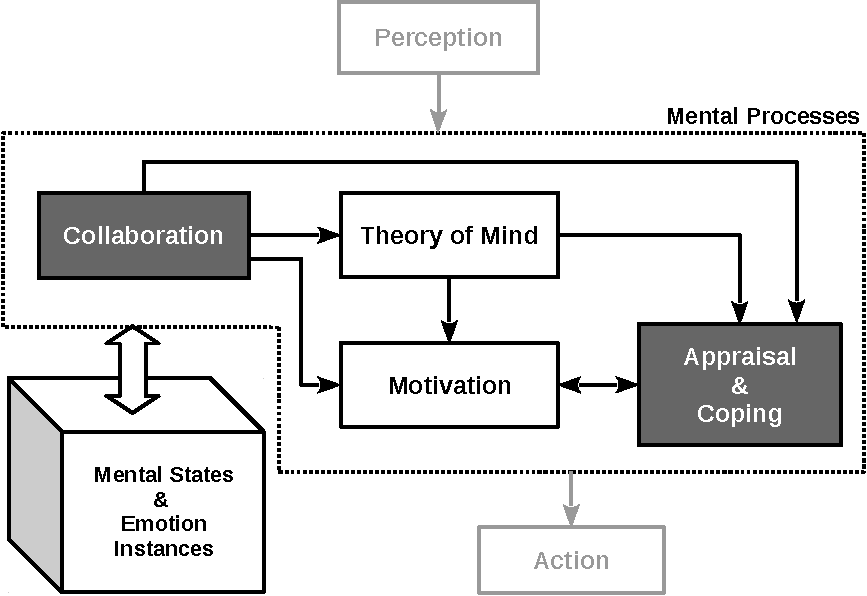
\includegraphics[width=0.45\textwidth]{figure/theory-general-croped.pdf}
  \caption{{\fontsize{9}{9}\selectfont Computational framework based on
  Affective Motivational Collaboration Theory (arrows indicate primary
  influences between mechanisms).}}
  \label{fig:cpm}
\end{figure}

Our focus is on the mechanisms depicted as mental processes in Figure
\ref{fig:cpm} along with the mental states. Each mechanism includes one our
more processes in our architecture. For instance, the \textit{Collaboration}
mechanism includes processes such as \textit{Focus Shifting} and
\textit{Constraint Management}, or as we discuss in Section
\ref{sec:appraisal-process} the \textit{Appraisal} mechanism includes processes
to compute the values for different appraisal variables. The \textit{mental
states} includes self's (robot's) beliefs, intentions, motives, goals and
emotion instances as well as the anticipated mental states of the other (human).
The \textit{Collaboration} mechanism maintains constraints on actions, including
task states and the ordering of tasks (see Figure \ref{fig:cs}). The
\textit{Collaboration} mechanism also provides processes to update and monitor
the shared plan. The \textit{Appraisal} mechanism is responsible for evaluating
changes in the self's mental states, the anticipated mental states of the other,
and the state of the collaboration environment. The \textit{Coping} mechanism
provides the self with different coping strategies associated with changes in
the self's mental states with respect to the state of the collaboration. The
\textit{Motivation} mechanism operates whenever the self a) requires a new
motive to overcome an internal impasse in an ongoing task, or b) wants to
provide an external motive to the other when the other faces a problem in a
task. The \textit{Theory of Mind} mechanism infers a model of the other's
anticipated mental state. The self progressively updates this model during the
collaboration.

\vspace*{-1mm}
\subsection{Mental States}
\label{sec:mental-states}

A brief description of mental states is provided as prerequisite knowledge for
understanding the appraisal processes. The mental states shown in Figure
\ref{fig:cpm} comprise the knowledge base required for all the mechanisms in the
overall model. Mental states are conscious states of the mind providing the
content for cognitive processes. Affective Motivational Collaboration Theory
operates with the following mental states: beliefs, intentions, motives, goals
and emotion instances. These mental states possess attributes, each of which
provides a discriminating and unique interpretation of the related cognitive
entities. The self uses these attributes whenever there is an arbitration in the
internal cognitive processes. We only describe the attributes of beliefs and
motives in this paper, since they are used in our appraisal algorithms. We do
not provide the way we compute the attributes' values, due to the limited space.

\vspace*{-2mm}
\subsubsection{Belief:}

\textit{Beliefs} are a crucial part of the mental states. We have two different
perspectives on categorization of beliefs. In one perspective, we categorize
beliefs based on whether they are shared between the collaborators. In the
second perspective, beliefs are categorized based on who or what they are about.
In this categorization, beliefs can be about the self, the other, or they can be
about the environment. Beliefs can be created and updated by different
processes. They also affect how these processes function as time passes.

The attributes of a belief are involved in arbitration procedures within
different processes in Affective Motivational Collaboration Theory. They impact
a range of these processes from the formation of new beliefs, the evaluation of
an external event by the Appraisal mechanism, generation of new motives and
updates on collaboration plan, to the activation of coping strategies and
ultimately the self's behavior. We use six belief attributes in our framework.
Belief \textit{strength} is about how strongly the self holds salient beliefs
about an object, an entity, or an anticipated behavior. \textit{Accuracy} of a
belief is the relation between that belief and the truth which that belief is
about. The \textit{frequency} of a belief is related to how regularly it appears
as the result of an internal or an external event. The \textit{recency} of a
belief refers to how temporally close a particular belief is to the current
state of collaboration. The \textit{saliency} of a belief is a cognitive
attribute that pertains to how easily the self becomes aware of a belief. The
\textit{persistence} of a belief refers to how resistant the belief is to
changes.

\vspace*{-2mm}
\subsubsection{Motive:}

\textit{Motives} are mental constructs which can initiate, direct and maintain
goal-directed behaviors. They are created by the emotion-regulated Motivation
mechanism. Motives can cause the formation of a new intention for the robot
according to: a) its own emotional states (how the robot appraises the
environment), b) its own private goal (how an action helps the robot to make
progress), c) the collaboration goal (how an action helps to achieve the shared
goal), and d) other's anticipated beliefs (how an action helps the other).
Motives can be compared on various dimensions \cite{sloman:motivation}, and
they possess a set of attributes. The Motivation mechanism compares motives
based on the quality of these attributes and chooses the one which is the most
related to the current state of the collaboration. We have the following five
motive attributes in our framework. The \textit{insistence} of a motive defines
the ``interrupt priority level'' of the motive, and how much that motive can
attract the self's focus of attention. The \textit{importance} of a motive is
determined by the corresponding beliefs about the effects of achieving or not
achieving the associated goal. The \textit{urgency} of a motive defines how much
time the self has to acknowledge and address that motive before it is too late.
The \textit{intensity} of a motive determines how actively and vigorously that
motive can help the self to pursue the goal if adopted; rather than abandoning
the goal and ultimately the collaboration. The \textit{failure disruptiveness}
attribute of a motive determines how disruptive failure is to achieving the
corresponding goal.

\vspace*{-2mm}
\subsubsection{Intention:}

\textit{Intentions} are mental constructs directed at goals and future actions.
They play an essential role in taking actions according to the collaboration
plan as well as behavior selection in the Coping mechanism. Intentions are
also involved in selecting intention-related strategies, e.g., planning, seeking
instrumental support and procrastination. Intentions possess a set of
attributes, i.e., \textit{Temporal Status, Direct Experience, Certainty,
Ambivalence, Affective-Deliberative Consistency} which moderate the consistency
between intention and behavior \cite{cooke:intention-behavior-consistency}. The
details about these attributes are out of this paper's context.

\vspace*{-2mm}
\subsubsection{Goal:}

\textit{Goals} help the robot to create and update its collaboration plan
according to the current private and shared goal content and structure, i.e.,
the \textit{Specificity, Proximity} and \textit{Difficulty} of the goal. Goals
direct the formation of intentions to take appropriate corresponding actions
during collaboration. Goals also drive the Motivation mechanism to generate
required motive(s). The details about goal's attributes are also out of this
paper's context.

\vspace*{-1mm}
\subsubsection{Emotion Instance:}

\textit{Emotions} in mental states are emotion instances that are elicited by
the Appraisal mechanism, e.g., \textit{Joy, Anger, Hope, Worry}. These emotion
instances include the robot's own emotions as well as the anticipated emotions
of the other which are created with the help of the processes in the Theory of
Mind mechanism. Each emotion has its own functionality in either the
intrapersonal or interpersonal level. These emotions not only regulate the
self's internal processes, but also assist the self to anticipate the other's
mental states.

\section{Example Scenario}

The example scenario is part of a much larger interaction we are implementing to
test our theory. This example shows a very short part of an interaction between
a robot and an astronaut during their collaboration. Their mission is to finish
installing a few solar panels together. However, the astronaut encounters a
measurement tool problem:

\vspace*{-1mm}
\begin{description}
  \item \textit{\textbf{\fontsize{9pt}{12pt}\selectfont Astronaut [turn t-1]:}}
  Oh no! Finishing the quality check of our installation with this measurement
  problem is so frustrating. I think we should stop now!

  \item \textit{\textbf{\fontsize{9pt}{12pt}\selectfont{Robot [turn t]:}}}
  \underline{I see. This is frustrating.} But, I can help you with the
  measurement tool and we can finish the task as originally planned.
\end{description}

\vspace*{-1mm}
As shown, the robot in turn $t$, acknowledges the astronaut's frustration and
appropriately responds to her problem. We will use this example in the Mental
Graph section to clarify some of the concepts. The underlined utterance of the
robot will be used in section Mental Graph.

\section{Collaboration}

The Collaboration mechanism constructs a hierarchy of goals associated with
tasks in the form of a hierarchical task network (see Figure \ref{fig:cs}), and
also manages and maintains the constraints and other required details of the
collaboration including the inputs and outputs of individual tasks, the
\textit{preconditions} (specifying whether it is appropriate to perform a task),
and the \textit{postconditions} (specifying whether a just-completed task was
successful). Collaboration also keeps track of the focus of attention, which
determines the salient objects, properties and relations at each point, and
shifts the focus of attention during the interaction.

\begin{figure}[tbh]
  \centering
  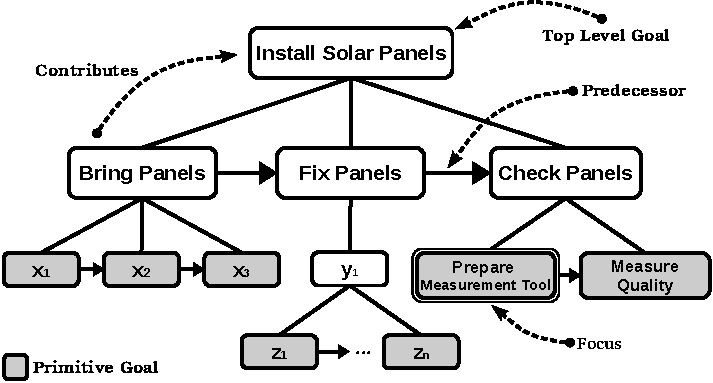
\includegraphics[width=0.474\textwidth]{figure/collaborationStructure-croped.pdf}
  \caption{{\fontsize{9}{9}\selectfont Collaboration structure (shared plan).}}
  \label{fig:cs}
\end{figure}

Here, we briefly describe the methods which retrieve information about the
collaboration structure, and are used in our algorithms to compute the values of
appraisal variables. In these methods, $\varepsilon_t$ is the event
corresponding to time \textit{t}, and $g_t$ is a given goal at time \textit{t}. 

\begin{itemize}
  \item \textit{recognizeGoal($\varepsilon_t$)} returns the unique goal to which
  the given event (action, utterance, or emotional expression) directly
  contributes, or \textit{ambiguous} if this method does not recognize a goal in
  the plan.
  \item \textit{topLevelGoalStatus($g_t$)} returns the status of the top level
  goal whether it is \textit{achieved, blocked} or \textit{in progress}. In
  our example, ``Install Solar Panels'' is the top level goal.
  \item \textit{currGoalStatus($g_t$)} returns the current goal status whe\-ther
  it is \textit{achieved, blocked, unknown} or \textit{in progress}. In our
  example, ``Prepare Measurement Tool'' is the current (focused) goal.
  \item \textit{precondStatus($g_t$)} returns the status of the precondition for
  the given goal whether it is \textit{satisfied, unsatisfied} or
  \textit{unknown}. For instance, the precondition for fixing a panel is whether
  the panel is appropriately located on its frame.
  \item \textit{doesContribute($g_t$)} returns whether the given goal
  contributes to another goal in the higher level of the plan hierarchy. For
  instance, an abstract (nonprimitive) goal of ``Bring Panels'' contributes to
  the higher level goal of ``Install Solar Panels''.
  \item \textit{extractContributingGoals($g_t$)} returns all the contributing
  goals of the given goal. For instance, the ``Prepare Measurement Tool'' and
  ``Measure Quality'' are two goals contributing to the ``Check Panels''
  nonprimitive goal.
  \item \textit{extractPredecessors($g_t$)} returns the predecessors of the
  given goal. For instance, the ``Prepare Measurement Tool'' goal is the
  predecessor of another goal called ``Measure Quality''.
  \item \textit{extractInputs($g_t$)} returns all the required inputs for
  the given goal. For example, the goal ``Fix Panels'' requires inputs such as
  the \textit{welding tool} and the \textit{panel}.
  \item \textit{isAvailable($g_t$)} returns whether the given input is
  available. For instance, if the \textit{welding tool} is required for the goal
  ``Fix Panels'', is it available now?
  \item \textit{isAchieved($g_t$)} returns whether the given goal is achieved,
  i.e., whether all the postconditions of the given goal are \textit{satisfied}.
  \item \textit{isFocused($g_t$)} returns whether the focus is on given
  goal now. The focus is on the goal ``Prepare Measurement Tool''. The focused
  goal is the goal that the robot currently is pursuing.
  \item \textit{getResponsible($g_t$)} returns responsible agents of the
  given goal. In a dyadic collaboration, both of the agents can be partly
  responsible for a nonprimitive goal, while each robot is responsible for one
  or more primitive goal. For instance, both the robot and the astronaut are
  responsible for the nonprimitive goal of ``Install Solar Panels'', whereas
  it is only the astronaut who is responsible for the primitive goal of
  ``Prepare Measurement Tool''.
\end{itemize}

\section{Mental Graph}
\label{sec:mental-graph}

In this section, we provide a graph representation of the robot's mental state
for the turn $t$ based on our example scenario. We only illustrate a part of the
robot's mental states in turn $t$ which is related to the event occurring based
on the astronaut's utterances in turn $t$-1. This section is provided because
all of our algorithms use mental graphs to compute values of appraisal
variables.

In Figure \ref{fig:mg}, we illustrate all five elements of robot's mental
states, i.e., belief, motive, intention, goal, and emotion, and the connections
between them. The belief node $b^{\{1,..,n\}}_{t-2}$ represents $n$ number of
beliefs that are carried over from the robot's previous mental state (shown as
one node for simplicity). These beliefs can be a combination of the robot's
private, inferred, and mutual beliefs as well as beliefs about self, other and
the environment. These beliefs have influence on motive formation and emotion
elicitation processes. However, there is another node representing belief
$b^{\varepsilon}_{t-1}$ which is the belief about the previous event
$\varepsilon_{t-1}$. In our example scenario, the astronaut's utterances in turn
$t$-1 concern a problem in a measurement tool and consequently her frustration,
which can lead to unsuccessful termination of the collaboration. The belief
about the previous event $\varepsilon_{t-1}$ also impacts the current motive
$m^{\delta}_t$ and emotion $e^{\delta}_t$. Note that the superscript $\delta$
used for motive $m^{\delta}_t$ and emotion $e^{\delta}_t$ indicates a specific
value for each of these mental states that is selected from among other possible
options based on an arbitration process. The motive $m^{\delta}_t$ (the need to
acknowledge the astronaut's emotion) leads to the formation of a required
intention $i_t$ (acknowledge astronaut's emotion) to achieve the current goal
$g_t$ (e.g., Prepare Measurement Tool).

In our algorithms, we use \textit{F{\fontsize{8}{8}\selectfont
IND}P{\fontsize{8}{8}\selectfont ATH}()} function to find the shortest path
between two given node. 

\begin{figure}
\begin{center}
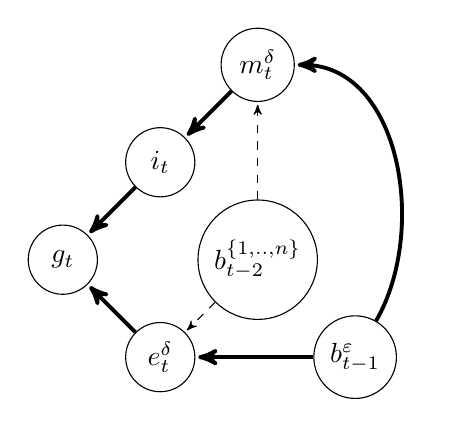
\begin{tikzpicture}[>=stealth',shorten >=1pt,node distance=1.75cm,on
grid,initial/.style    ={}] 
  \node[state]          (G)                         {$g_t$};
  \node[state]          (I1) [above right =of G]    {$i_t$};
  \node[state]          (E1) [below right =of G]    {$e^{\delta}_t$};
  \node[state]          (M1) [above right =of I1]   {$m^{\delta}_t$};
  \node[state]          (B1) [below right =of I1]   {$b^{\{1,..,n\}}_{t-2}$};
  \node[state]          (B2) [below right =of B1]   {$b^{\varepsilon}_{t-1}$};
\tikzset{mystyle/.style={->,double=black}}
\tikzset{every node/.style={fill=black}} 
\path (M1)    edge [mystyle]   (I1) 
      (B2)    edge [mystyle]   (E1)
      (I1)    edge [mystyle]   (G)
      (E1)    edge [mystyle]   (G);
\tikzset{mystyle/.style={->,dashed=black}}
\path (B1)    edge [mystyle]   (E1) 
      (B1)    edge [mystyle]   (M1);
\tikzset{mystyle/.style={->,relative=false,in=0,out=60,double=black}}
\path (B2)    edge [mystyle]   (M1); 
\end{tikzpicture}
\caption{{\fontsize{9}{9}\selectfont Abstract structure of robot's mental graph
in turn $t$.}}
\label{fig:mg}
\end{center}
\vspace*{-6mm}
\end{figure}

\vspace*{-2mm}
\section{Appraisal Processes}
\label{sec:appraisal-process}

All of the algorithms in this section use a mental graph which is a directed
acyclic graph constructed based on the mental states of the robot at each turn
during the collaboration. They also use the content of the most recent event at
each turn. We consider four appraisal variables to be the most important
variables in a collaboration context, i.e., \textit{Relevance} (Algorithm
\ref{alg:relevance}), \textit{Desirability} (Algorithm \ref{alg:desirability}),
\textit{Expectedness} (Algorithm \ref{alg:expectedness}), and
\textit{Controllability} (Algorithm \ref{alg:controllability}). There are other
appraisal variables introduced in psychological
\cite{scherer:appraisal-processes} and computational literature
\cite{gratch:domain-independent}. We believe most of these variables can be
straightforwardly added to our appraisal mechanism later.

\subsection{Relevance}

Relevance as an appraisal variable measures the significance of an event for the
robot. An event can be evaluated to be relevant if it has a positive utility or
it can causally impact a state with a positive utility
\cite{marsella:ema-process-model}. Relevance is an important appraisal variable
since the other appraisal variables are only computed for the relevant events.

Algorithm \ref{alg:relevance} determines the relevance of the given event with
respect to the current mental state. An event is \textit{irrelevant} if there is
no connection between the event and the current shared goal. If there is a
connection, the relevance of the event will depend on the significance of the
event with respect to the current collaboration status. The significance of an
event is determined based on the utility of the event as it is also presented in
\cite{gratch:domain-independent,marsella:ema-process-model}. We believe although
the utility of the event represents the significance of the event, the other
collaborator's expressed emotion also plays a role by influencing the
significance of the utility through a threshold. As a result, evaluating the
relevance of the events can cause a collaborative robot to effectively respond
only to the events which can positively impact the status of the shared goal
without dedicating all other resources to every single event. The relevance
process also benefits from the information that the collaboration structure
contains, e.g., shared goal.

After perceiving an event, it is the belief about that event which represents
the event in robot's mental state (line 2). $g_{t}$ (line 3) represents the
shared goal (in the mental graph) at time (turn) $t$ within the shared plan.
Then, we find the shortest path ($\mathcal{P}$) between the nodes
$\mathit{b}_{\varepsilon_t}$ and $g_{t}$ in the mental graph. If there is no
path, the algorithm finds the event \textit{irrelevant} and terminates.

\begin{algorithm}
	\caption{(Relevance)}
	\label{alg:relevance}
	\begin{algorithmic}[1]
		\Function{IsEventRelevant}{{\fontsize{8.0}{9}\selectfont MentalGraph}
		$\mathcal{G}_{t}$, {\fontsize{8.5}{9}\selectfont Event} $\varepsilon_t$}
			\Statex
			\State $\mathit{b}_{\varepsilon_t} \gets \Call{getBelief}{\varepsilon_t}$
			\State $\mathit{g}_{t} \gets \textit{currGoal}{(\mathcal{G}_{t})}$
			\Statex
			\State $\mathcal{P} \gets \Call{findPath}{\mathit{b}_{\varepsilon_t},
			\mathit{g}_{t}}$
			\Statex
			\If {$(\mathcal{P} = \emptyset)$}
				\State \Return {{\fontsize{8}{8}\selectfont IRRELEVANT}}
			\Else
				\State $\mathcal{U} \gets \Call{getEventUtility}{\mathit{b}_{\varepsilon_t},
				\mathit{g}_{t}}$ 
				\State $\tau_{t} \gets \Call{getEmotionalThreshold}{\mathcal{G}_{t}}$
				\If {$( \mathcal{U} \geq \tau_{t} )$}
				\State \Return {{\fontsize{8}{8}\selectfont RELEVANT}}
				\Else
					\State \Return {{\fontsize{8}{8}\selectfont IRRELEVANT}}
				\EndIf
			\EndIf
		\EndFunction
	\end{algorithmic}
\end{algorithm}

However, if there is a path between $\mathit{b}_{\varepsilon_t}$ and $g_{t}$, we
need a way to determine whether the event is relevant. First, we compute the
utility $(\mathcal{U})$ of the event ($0 \leq \mathcal{U} \leq 1$)
based on the values of the attributes associated with
$\mathit{b}_{\varepsilon_t}$, as well as the attributes of the motive within the
path $\mathcal{P}$. The significance of an event in a collaborative environment
is based not only on the utility of the event, but it is also influenced by the
perceived emotion of the human collaborator. The human's emotion influences the
decision about the utility of the event in form of a threshold value
($\tau_{t}$). For instance, a positive expressed emotion of the human reduces
the threshold value which consequently makes the robot find an event relevant
with even a slightly positive utility.

We compute this threshold value ($\tau_{t}$) using a Fuzzy Logic system on a
three-dimensional space of the somatic markers associated with the other's
expressed emotion as they are described in \cite{breazeal:sociable-robot}. In
this space every emotion can be mapped to a vector of three values, i.e.,
\textit{Arousal, Valence} and \textit{Stance}. The details about this process is
out of this paper's context. Finally, we make our decision about the relevance
of an event with respect to the human's emotional state. Consequently, an event
can be considered \textit{irrelevant} even though there is a path between
$\mathit{b}_{\varepsilon_t}$ and $g_{t}$.

\subsection{Desirability}

Desirability characterizes the value of an event to the robot in terms of
whether the event facilitates or thwarts the collaboration goal. Desirability
captures the valence of an event with respect to the robot's preferences
\cite{gratch:domain-independent}. In a collaborative robot, preferences are
biased towards those events facilitating progress in the collaboration. An event
is desirable if it facilitates the state of the shared goal, or if it inhibits
the state of a goal that is inconsistent with respect to the shared goal.

\begin{algorithm}
	\caption{(Desirability)}
	\label{alg:desirability}
	\begin{algorithmic}[1]
		\Function{IsEventDesirable}{{\fontsize{7.5}{8}\selectfont
		MentalGraph $\mathcal{G}_{t}$}, {\fontsize{7.5}{8}\selectfont Event $\varepsilon_t$}}
			\Statex
			\If {{\fontsize{8}{9}\selectfont(\textit{topLevelGoalStatus($g_{t}$)} =
			{\fontsize{7}{8}\selectfont ACHIEVED})}} 
			\State \Return {{\fontsize{7}{8}\selectfont HIGH-DESIRABLE}} 
			\ElsIf {{\fontsize{8}{9}\selectfont(\textit{topLevelGoalStatus($g_{t}$)}} =
			{\fontsize{7}{8}\selectfont FAILED})} 
			\State \Return {{\fontsize{7}{8}\selectfont HIGH-UNDESIRABLE}}
			\ElsIf {{\fontsize{8}{9}\selectfont(\textit{topLevelGoalStatus($g_{t}$)}} =
			{\fontsize{7}{8}\selectfont BLOCKED}) \OR
			\hspace{1mm}{\fontsize{8}{9}\selectfont
			\hspace*{5mm}(\textit{topLevelGoalStatus($g_{t}$)}} =
			{\fontsize{7}{8}\selectfont INAPPLICABLE})}
			\State \Return {{\fontsize{7}{8}\selectfont UNDESIRABLE}} 
			\ElsIf {{\fontsize{8}{9}\selectfont(\textit{topLevelGoalStatus($g_{t}$)}} =
			{\fontsize{7}{8}\selectfont PENDING}) \OR
			\hspace{1mm}{\fontsize{8}{9}\selectfont
			\hspace*{5mm}(\textit{topLevelGoalStatus($g_{t}$)}} =
			{\fontsize{7}{8}\selectfont INPROGRESS})}
				\Statex
				\If {{\fontsize{8}{9}\selectfont (\textit{currGoalStatus($g_{t}$)}} =
				{\fontsize{7}{8}\selectfont ACHIEVED})}
				\State \Return {{\fontsize{7}{8}\selectfont DESIRABLE}}
				\ElsIf {(\textit{currGoalStatus($g_{t}$)} = {\fontsize{7}{8}\selectfont
				FAILED})} 
				\State \Return {{\fontsize{7}{8}\selectfont HIGH-UNDESIRABLE}}
				\ElsIf {(\textit{currGoalStatus($g_{t}$)} = {\fontsize{7}{8}\selectfont
				BLOCKED}) \OR 
				\hspace{1mm}{\fontsize{8}{9}\selectfont
				\hspace*{10mm}(\textit{topLevelGoalStatus($g_{t}$)}} =
				{\fontsize{7}{8}\selectfont INAPPLICABLE})} 
				\State \Return {{\fontsize{7}{8}\selectfont UNDESIRABLE}}
				\ElsIf {{\fontsize{8}{9}\selectfont(\textit{topLevelGoalStatus($g_{t}$)}} =
				{\fontsize{7}{8}\selectfont PENDING}) \OR \hspace{1mm} 
				\hspace*{10mm}(\textit{currGoalStatus($g_{t}$)} =
				{\fontsize{7}{8}\selectfont INPROGRESS})} 
				\State \Return {{\fontsize{7}{8}\selectfont NEUTRAL}}
				\EndIf
			\EndIf
		\EndFunction
	\end{algorithmic}
\end{algorithm}

Desirability plays an important role in the overall architecture; it makes the
processes involved in the other mechanisms (e.g., Motivation and Theory of
Mind), and consequently the robot's mental state, congruent with the
collaboration status which is the robot's desire. Therefore, it causes the robot
to dismiss events causing inconsistencies in the robot's collaborative behavior.
Moreover, desirability is also crucial from the collaboration's point of view. A
collaborative robot needs to know whether its own and the other collaborator's
actions, utterances, and emotional expressions are desirable in terms of their
consistence with the status of the current shared goal. In other words, the
collaboration mechanism uses the appraisal process of desirability to coordinate
what the self or the other does, says, and expresses during collaboration.
Reciprocally, the appraisal mechanism and in this case the desirability process
use the collaboration structure to obtain their required information.

Algorithm \ref{alg:desirability} provides a process in which the desirability of
an event is computed with regard to the status of the shared goal; i.e., it
operates based on whether and how the event changes the status of the current
shared goal. It receives the current mental graph, $\mathcal{G}_{t}$, and the
current event, $\varepsilon_t$, and decides whether and how the event is
desirable or undesirable. First, the algorithm checks the status of the
collaboration's top level goal (lines 2 to 6), and if the the top level goal is
still in progress, it continues by checking the status of the current shared
goal (lines 7 to 13). If any of the top level and current shared goals are
achieved in these two steps, the robot interprets the event as a desirable one.
However, if any of these goals are blocked, the event will be considered
undesirable by the robot.

The algorithm continues in the case of an unknown status of the current shared
goal, and checks whether the precondition(s) of the associated goal with the
current event, $\mathit{g}_{\varepsilon_t}$, are satisfied (lines 17 to 21).
The robot prefers the satisfied preconditions and interprets the event as
desirable while unsatisfied preconditions are undesirable for the robot. For
instance, a satisfied precondition of a future goal is still desirable for the
robot to some extent. Note that the robot also checks the ambiguity of the
associated goal with the current event (line 15). An ambiguous goal is a goal
which is not recognized in the robot's plan, and it is undesirable for the
robot. Finally, if the preconditions of the associated goal with the current
event are unknown, the robot checks whether this goal,
$\mathit{g}_{\varepsilon_t}$, contributes to the current shared goal,
$\mathit{g}_{t}$ (lines 22 to 25). As a result a contributing goal will obtain a
neutral desirability in comparison with a noncontributing goal which will be
undesirable for the robot.

\subsection{Expectedness}

Expectedness is the extent to which the truth value of a state could have been
predicted from causal interpretation of an event
\cite{marsella:ema-process-model}. In the collaboration context the expectedness
of an event measures the congruency of the event with respect to the existing
knowledge about the shared goal. Therefore, expected events are those of which
beliefs about them are congruent to the status of the collaboration since their
associated goals are expected with respect to the shared plan.

Expectedness underlies a collaborative robot's attention by evaluating the
congruence of events with respect to the structure of an existing shared plan.
Congruent beliefs in a robot's mental state will lead to more consistent and
effective outcomes of the processes in the overall architecture. Therefore,
a collaborative robot uses expectedness to maintain its own mental state towards
the shared goal. The robot will also be able to respond to unexpected but
relevant events. As a result, the collaboration mechanism uses expectedness to
maintain the robot's attention and subsequently its mental state with respect to
the shared goal. In parallel, the appraisal mechanism uses the underlying
information of the collaboration structure to evaluate the expectedness of an
event.

\begin{algorithm}
	\caption{(Expectedness)}
	\label{alg:expectedness}
	\begin{algorithmic}[1]
		\Function{IsEventExpected}{{\fontsize{8}{9}\selectfont MentalGraph}
		$\mathcal{G}_{t}$, {\fontsize{8}{9}\selectfont Event} $\varepsilon_t$}
			\Statex
			\State $\mathit{g}_{t} \gets \textit{recognizeGoal}{(\varepsilon_t)}$
			\State $\mathit{g}_{top} \gets \textit{getTopGoal}{(\mathit{g}_{t})}$
			\Statex
			\If {$(\textit{isLive}{(\mathit{g}_{t})})$}
				\If {$(\textit{isNeccessaryFocusShift}{(\mathit{g}_{t})})$}
					\State \Return {\fontsize{8}{8}\selectfont MOST-EXPECTED}
				\Else
					\State \Return {\fontsize{8}{8}\selectfont EXPECTED}
				\EndIf
			\Else
				\If {$(\textit{isPath}{(\mathit{g}_{t}, \mathit{g}_{top})})$}
					\State \Return {\fontsize{8}{8}\selectfont UNEXPECTED}
				\Else
					\State \Return {\fontsize{8}{8}\selectfont MOST-UNEXPECTED}
				\EndIf
			\EndIf
		\EndFunction
	\end{algorithmic}
\end{algorithm}

In Algorithm \ref{alg:expectedness} we provide the process of the expectedness
based on the shared plan and status of the shared goal. The key point in this
algorithm is the status of the current shared goal ($\mathit{g}_{t}$) and its
relationship with the goal associated with the current event 
($\mathit{g}_{\varepsilon_t}$).  The algorithm receives the current mental
graph, $\mathcal{G}_{t}$, and the current event, $\varepsilon_t$, from input,
and decides whether the current event is expected. 

First, we need to extract the goal in the current mental graph and the
recognized goal associated with the current event. Similar to the desirability
algorithm (Algorithm \ref{alg:desirability}), we check whether the
$\mathit{g}_{\varepsilon_t}$ is ambiguous. In the case of ambiguity in
$\mathit{g}_{\varepsilon_t}$, we consider the current event unexpected since an
effective collaboration requires perceivable and unambiguous goals associated
with the events. We continue by the comparison of the current shared goal and
the recognized goal associated with the current event with respect to the shared
plan. If these two goals are not the same, it is possible that the current
shared goal is already achieved. The event will be unexpected (line 10) if the
current shared goal is not achieved and the current event does not refer to the
same goal. However, if the current goal is achieved, it is important to see
whether its parent is also achieved (line 12). This step is important because
the event can be expected if the new goal contributes to the parent of the
recently achieved goal. Therefore, if the parent goal in the hierarchical plan
is not achieved, the contribution of the associated goal to the current event
can help us to decide whether the event is expected (lines 12 to 16). However,
if the parent goal is already achieved, the new goal can contribute (as a child)
to the recently achieved shared goal, i.e., $\mathit{g}_{t}$, which is also
expected (line 19). On the contrary, if the new goal does not contribute to
$\mathit{g}_{t}$, it might be a goal in another branch in the shared plan which
has received focus and should be achieved. In such a case, again, the event will
be expected; otherwise we consider the event unexpected (lines 21 to 24).

\vspace*{-2mm}
\subsection{Controllability}

Controllability is the extent to which an event can be influenced, and it is
associated with a robot's ability to cope with an appraised event
\cite{gratch:domain-independent}. Thus, a robot can determine whether the
outcome of an event can be altered by some actions under either of the
collaborators' control. In other words, controllability is a measure of a
robot's ability to maintain or change a particular state as a consequence of an
event.

\begin{algorithm}
	\caption{(Controllability)}
	\label{alg:controllability}
	\begin{algorithmic}[1]
		\Function{IsEventControllable}{Event $\varepsilon_t$}
			\Statex
			\State $\alpha \gets \Call{GetAgencyRatio}{\varepsilon_t}$ 
			\State $\beta \gets \Call{GetAutonomyRatio}{\varepsilon_t}$
			\Statex
			\State $\lambda \gets
			\Call{\small{GetSucPredecessorsRatio}}{\varepsilon_t}$
			\State $\mu \gets
			\Call{\small{GetAvailableInput}}{\varepsilon_t}$
			\Statex
			\State $\mathcal{U} \gets
			\frac{\omega_{0}\cdot \alpha + \omega_{1}\cdot \beta + \omega_{2}\cdot
			\lambda + \omega_{3}\cdot \mu}{\omega_{0} + \omega_{1} + \omega_{2} +
			\omega_{3}}$
			\Statex
			\State $\tau_{t} \gets \Call{getEmotionalThreshold}{ }$
			\Statex
			\If {$(\mathcal{U} \geq \tau_t)$}
				\State \Return {{\fontsize{8}{8}\selectfont CONTROLLABLE}}
			\Else
				\State \Return {{\fontsize{8}{8}\selectfont UNCONTROLLABLE}}
			\EndIf
		\EndFunction
	\end{algorithmic}
\end{algorithm}

Controllability is also important for the overall architecture. For instance,
the robot can choose to ask or negotiate about a collaborative task which is
not controllable; it can cause the robot to interpret or predict the other's
emotional state (e.g., anger if the task is blocked, i.e., uncontrollable for
the other), or form a new motive to establish an alternative goal for the
current uncontrollable event. In general, other mechanisms in the architecture
use the appraisal process of controllability in their decision making processes;
meanwhile controllability uses the information from the collaboration structure,
e.g., successful predecessors of a goal.

An important determinant of one's emotional response is the sense of control
over the events occurring. This sense of subjective control is based on one's
reasoning about self's power. For instance, the robustness of one's plan for
executing actions can increase sense of power and subsequently the sense of
control. In the collaboration context, we have translated the sense of control
into a combination of four different factors including a) \textit{agency} and b)
\textit{autonomy} of the robot, as well as the ratios of c) \textit{successful
predecessors}, and d) the \textit{available inputs} of a given goal
(i.e., $\mathit{g}_{\varepsilon_t}$) in the shared plan.

In Algorithm \ref{alg:controllability}, we compute the controllability of an
event based on these four factors (lines 2 to 5). Algorithms \ref{alg:agency} to
\ref{alg:inputs} are used to illustrate the underlying processes of all these
factors. We use weighted averaging over these four factors to compute the
utility of an event in terms of controllability of the event. However, the
value of all these weights are set to 1.0 for the purpose of simplicity at
this stage of the project. We will adjust these weights after further
investigating the influence of these factors, and implementing other mechanisms
in the overall architecture. After computing the value of the utility, we
compare this value to an emotional threshold similar to what we discussed in
Algorithm \ref{alg:relevance}. This comparison leads to our decision about the
controllability of an event (lines 8 to 11).

\renewcommand\thealgorithm{4\alph{algorithm}}
\setcounter{algorithm}{0}

\begin{algorithm}
	\caption{(Get Agency Ratio)}
	\label{alg:agency}
	\begin{algorithmic}[1]
		\Function{GetAgencyRatio}{Event $\varepsilon_t$}
			\Statex
			\State $\mathit{g}_{t} \gets \textit{recognizeGoal}{(\varepsilon_t)}$
			\Statex
			\State $\mathcal{M}_{t} \gets \textit{getActiveMotive}{(\mathit{g}_{t})}$
			\Statex
			\If {$(\mathcal{M}_{t} \neq \emptyset)$}
				\If {$(\mathcal{M}_{t}\cdot type = $
				{{\fontsize{8}{8}\selectfont INTERNAL}}$)$} \State \Return {1.0}
				\Else
					\State \Return {0.0}
				\EndIf
			\Else
				\State \Return {0.0}
			\EndIf
		\EndFunction 
	\end{algorithmic}
\end{algorithm}

\vspace*{-3mm}
Agency is the capacity of an individual to act independently in any given
environment. In a collaborative environment sometimes collaborators are required
to act independently of each other. Hence, they need to have some internal motives
that are formed based on their own mental state rather than being reinforced by
the other. These internal motives will lead the collaborators to acquire new
intentions towards new goals whenever it is required. In Algorithm
\ref{alg:agency}, if there is a path between the belief about the current event
and the recognized goal associated with that event, we extract the motive within
the acquired path. We consider maximum agency value denoted as $\alpha$ in
Algorithm \ref{alg:controllability} (i.e., $\alpha=1.0$) if the robot's mental
state possesses an internal motive towards the recognized goal; otherwise we
consider the minimum agency value (i.e., $\alpha=0.0$) for no motives or
external motives only. Note that the process of forming new internal motives is
out of this paper's context.

\renewcommand\thealgorithm{4\alph{algorithm}}
\setcounter{algorithm}{1}

\begin{algorithm}
	\caption{(Get Autonomy Ratio)}
	\label{alg:autonomy}
	\begin{algorithmic}[1]
		\Function{GetAutonomyRatio}{Event $\varepsilon_t$}
			\Statex
			\State $\mathit{g}_{t} \gets \textit{recognizeGoal}{(\varepsilon_t)}$
			\Statex
			\State $\Phi_{\mathit{g}} \gets
			\textit{extractContributingGoals}{(\mathit{g}_{t})}$
			\Statex
			\ForAll {$\phi_{\mathit{g}}^i \in \Phi_{\mathit{g}}$}
				\If {$(\textit{getResponsible}{(\phi_{\mathit{g}}^i)} =$
				{\fontsize{8}{8}\selectfont SELF})} 
					\State $count_{self} \gets count_{self} + 1$
				\EndIf
			\EndFor
			\Statex
			\State \Return 
			${count_{self} \mathbin{/} {{\Phi_{\mathit{g}}}.total()}}$
		\EndFunction 
	\end{algorithmic}
\end{algorithm}

Autonomy is the ability to make decisions without the influence of others.
Autonomy implies acting on one's own and being responsible for that. In a
collaborative environment, tasks are delegated to the collaborators based on
their capabilities. Therefore, each collaborator is responsible for the
delegated task and the corresponding goal. In Algorithm
\ref{alg:controllability}, $\beta$ denotes the value of autonomy with regard to
the event ($\varepsilon_t$). This value is the ratio of the number of the
contributing goals to $\mathit{g}_{\varepsilon_t}$ for which the robot is
responsible over the total number of contributing goals to
$\mathit{g}_{\varepsilon_t}$ (see Algorithm \ref{alg:autonomy}). If the
goal associated with the current event corresponds to a nonprimitive task, the
algorithm checks the responsible agent for each primitive task contributing to
the nonprimitive one and returns a value of which $(0 \leq \beta \leq 1)$.
However, if the associated goal of the current event corresponds to a primitive
task the value of $\beta$ would be 0 or 1. In general, higher autonomy leads to
a more positive value of controllability.

\renewcommand\thealgorithm{4\alph{algorithm}}
\setcounter{algorithm}{2}

\begin{algorithm}
	\caption{(Get Succeeded Predecessors Ratio)}
	\label{alg:predecessors}
	\begin{algorithmic}[1]
		\Function{GetSucPredecessorsRatio}{Event $\varepsilon_t$}
			\Statex
			\State $\mathit{g}_{t} \gets \textit{recognizeGoal}{(\varepsilon_t)}$
			\Statex
			\State $\Theta{\mathit{g}} \gets
			\textit{extractPredecessors}{(\mathit{g}_{t})}$
			\Statex
			\ForAll {$\theta_{\mathit{g}}^i \in \Theta_{\mathit{g}}$}
				\If {$(\textit{isAchieved}{(\theta_{\mathit{g}}^i)})$}
					\State $count_{achieved} \gets count_{achieved} + 1$
				\EndIf
			\EndFor
			\Statex
			\State \Return
			${count_{achieved} \mathbin{/} {\Theta{\mathit{g}}.total()}}$
		\EndFunction 
	\end{algorithmic}
\end{algorithm}

\vspace*{-3mm}
The structure of a shared plan accommodates the order of the required
predecessors of a goal. Predecessors of a goal, $g$, are other goals that
the collaborators should achieve before trying to achieve goal $g$. In Algorithm
\ref{alg:predecessors}, we use the ratio of successfully achieved predecessors
of the recognized goal ($\mathit{g}_{\varepsilon_t}$) associated with the
current event over the total number of predecessors of the same goal. This ratio
(denoted as $\lambda$ in Algorithm \ref{alg:controllability}) is another factor
used to compute the controllability of an event. If all of the predecessors of
the given goal are already achieved, then $\lambda=1$ which is the maximum value
for $\lambda$. On the contrary, failure of all of the predecessors will lead to
$\lambda=0$. Therefore, higher $\lambda$ value positively impacts the value of
controllability for the current event.

\renewcommand\thealgorithm{4\alph{algorithm}}
\setcounter{algorithm}{3}

\begin{algorithm}
	\caption{(Get Available Input Ratio)}
	\label{alg:inputs}
	\begin{algorithmic}[1]
		\Function{GetAvailableInputRatio}{Event $\varepsilon_t$}
			\Statex
			\State $\mathit{g}_{t} \gets \textit{recognizeGoal}{(\varepsilon_t)}$
			\Statex
			\State $\mathcal{X}_{\mathit{g}} \gets
			\textit{extractInputs}{(\mathit{g}_{t})}$
			\Statex
			\ForAll {$\chi_{\mathit{g}}^i \in \mathcal{X}_{\mathit{g}}$}
				\If {$(\textit{IsAvailable}{(\chi_{\mathit{g}}^i)})$}
					\State $count_{available} \gets count_{available} + 1$
				\EndIf
			\EndFor
			\Statex
			\State \Return
			${count_{available} \mathbin{/} \mathcal{X}_{\mathit{g}}.total()}$
		\EndFunction 
	\end{algorithmic}
\end{algorithm}

Inputs of a task are the required elements that the collaborators use to
achieve the specified goal of the task. These inputs are also part of the
structure of a shared plan. In Algorithm \ref{alg:inputs}, we extract the
required inputs of the associated goal with the current event, and check whether
all the required inputs are available for the goal $\mathit{g}_{\varepsilon_t}$.
The outcome will be the ratio of the available required inputs over the total
required inputs of the goal associated with the current event. This value
(denoted as $\mu$ in Algorithm \ref{alg:controllability}) will be bound to 0 and
1. Similar to the other factors in the controllability process, the closer the
value of $\mu$ gets to 1, the more positive impact it has on the overall
controllability value of the event.

\vspace*{-3mm}
\section{Evaluation}
\label{sec:user-study}

We conducted a between subject user study using an online crowdsourcing
website -- CrowdFlower\footnote{http://www.crowdflower.com}. Each group
originally had 40 subjects. To increase the quality of our subjects' answers, we
limited the visibility of our questionnaires to a few English speaking
countries, i.e., United States, Britain, and Australia. We also limited our
subject pools to those that have acquired the highest confidence level on the
crowdsourcing website. Our questionnaires included 2 or 3 test questions
(depending on the length) to check the sanity of the answers. We eliminated
subjects providing wrong answers to our test questions. We also eliminated
subjects with an answering time less than 2 minutes. The final number of
accepted subjects in each group is provided in Table \ref{tbl:statistics}.

\begin{figure}[tbh]
  \centering
  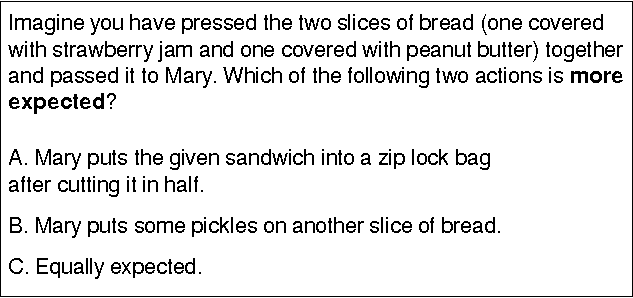
\includegraphics[width=0.425\textwidth]{figure/question-sample-croped.pdf}
  \caption{{\fontsize{9}{9}\selectfont An example question from the expectedness
  questionnaire.}}
  \label{fig:qs}
\end{figure}

To minimize the background knowledge necessary, we used a simple domestic
example of preparing a peanut butter and jelly sandwich, and a hard boiled egg
sandwich for a hiking trip. We provided clear textual and graphical instructions
for all four questionnaires. The instructions focused on hypothetical
collaboration between the test subject and an imaginary friend, Mary; their goal
was to prepare two sandwiches. We also provided a brief description as well as a
simple example for each appraisal variable, e.g., \textit{relevance}, at the end
of the corresponding instructions. We prepared four different online
questionnaires for the appraisal variables: \textit{relevance, desirability,
expectedness} and \textit{controllability}. All these questions were designed
based on different parameters that we use in our algorithms (see Section
\ref{sec:appraisal-process}). Each question provided three options. One option
provided a distinct alternative; another option was used to provide a dichotomy
with the first alternative, and a third option was used to check whether the
subjects perceived the other two options as equal. Figure \ref{fig:qs} shows an
example question from one of our questionnaires.

We conducted the user study to compare the results with the implemented
algorithms discussed in Section \ref{sec:appraisal-process}. As we mentioned,
each question had 3 answers. Therefore, a totally random distribution would
result in 33\% agreement with our algorithms results. However, the average
ratio indicating similarity between human subjects decisions and the output of
our algorithms is significantly higher than 33\%. The total number of subjects'
answers similar to a) the \textit{relevance} algorithm (n=29) averaged 71.3\%
(s=10.7\%), b) the \textit{desirability} algorithm (n=35) averaged 77.8\%
(s=15.0\%), c) the \textit{expectedness} algorithm (n=33) averaged 78.5\%
(s=12.0\%), and d) the \textit{controllability} algorithm (n=33) averaged 74.3\%
(s=15.8\%). It is worth noting that the human subjects agreed 100\% on some
questions, while one some other questions there was a much lower level of
agreement.

\begin{table}
\centering
\caption{Results From Our User Study}
\begin{tabular}{|c|c|c|c|c|} \hline
{\fontsize{7.5}{8}\selectfont Appraisal Variables} &
{\fontsize{7.5}{8}\selectfont \# of Subjects} & {\fontsize{8}{8}\selectfont
Mean} & {\fontsize{7.5}{8}\selectfont Stdev} &
{\fontsize{7.5}{8}\selectfont\textit{p}-value}\\ \hline 
{\fontsize{7.5}{8}\selectfont Relevance} & 29 & 0.713 & 0.107 & <0.001\\ \hline
{\fontsize{7.5}{8}\selectfont Desirability} & 35 & 0.778 & 0.150 & <0.001\\
\hline 
{\fontsize{7.5}{8}\selectfont Expectedness} & 33 & 0.785 & 0.120 & <0.001\\
\hline 
{\fontsize{7.5}{8}\selectfont Controllability} & 33 & 0.743 & 0.158 & <0.001\\
\hline
\end{tabular}
\label{tbl:statistics}
\vspace*{-7mm}
\end{table}

The results indicate that our algorithms provide a sufficiently accurate
representation of human's appraisal. The \textit{p}-values obtained based on a
one-tailed z-test (see Table \ref{tbl:statistics}) show the probability of
human subjects' data being generated from a random set. The very small
\textit{p}-values indicate that the data set is not random; in fact, the high
percentage of similarity shows it is strongly inclined towards the four
appraisal algorithms.

These results indicate that there is a similarity between human subjects'
answers and the results from our appraisal algorithm. However, if human subjects
thought exactly the same as our algorithms' decision processes, the average
number of similarity to our result would be 100\%. We believe the difference between
these two results could be because of several reasons, including: a) the fact
that we conducted our study online and had less control on our subjects, b) our
algorithms might require further granularity, c) the difference between decision
making processes of individuals, which can be affected by other factors such as
personality, gender, and culture. While it maybe possible to achieve a higher
level of agreement between humans and the algorithms results, these results
indicate that the current algorithms are adequate to be used in collaboration
context.

% end the environment with {table*}, NOTE not {table}!

%Note that either {\textbf{.ps}} or {\textbf{.eps}} formats are
%used; use
%the \texttt{{\char'134}epsfig} or \texttt{{\char'134}psfig}
%commands as appropriate for the different file types.

%\end{document}

%Acknowledgements are optional
\section*{Acknowledgments}

%
%APPENDICES are optional
%\balancecolumns
%Appendix A
%
% For AAMAS-2016, as references are unlimited but appendices must fit within
% 8 pages, the References section must come after the appendices (if any)
%
% The following two commands are all you need in the
% initial runs of your .tex file to
% produce the bibliography for the citations in your paper.
\bibliographystyle{abbrv}
\bibliography{mshayganfar.bib}  % sigproc.bib is the name of the Bibliography in this case
% You must have a proper ".bib" file
%  and remember to run:
% latex bibtex latex latex
% to resolve all references
%
% ACM needs 'a single self-contained file'!
%\balancecolumns % GM June 2007
% That's all folks!
\end{document}
